% AnyCam paper draft. On Overleaf the Elsevier class (elsarticle) is used automatically;
% without it (e.g. a local TeX install) the same file compiles with the standard article class.
\newif\ifels
\IfFileExists{elsarticle.cls}{\elstrue}{\elsfalse}
\ifels
  \documentclass[preprint,12pt,authoryear]{elsarticle}
  \def\bibsty{elsarticle-harv}
\else
  \documentclass[11pt]{article}
  \usepackage[a4paper,margin=2.5cm]{geometry}
  \usepackage[authoryear,round]{natbib}
  \def\bibsty{plainnat}
  \newenvironment{frontmatter}{}{}
  \newcommand{\journal}[1]{}
  \newcommand{\affiliation}[1]{\date{#1}}
  \newcommand{\sep}{; }
  \renewenvironment{abstract}{\maketitle\section*{Abstract}}{}
  \newenvironment{keyword}{\par\noindent\textbf{Keywords:} }{\par}
\fi
\usepackage[T1]{fontenc}
\usepackage{amsmath,amssymb}
\usepackage{graphicx}
\usepackage{booktabs}
\usepackage{multirow}
\usepackage{xcolor}
\usepackage[hidelinks]{hyperref}
\usepackage{caption}
\captionsetup{font=small,labelfont=bf}
\newcommand{\pending}{\textcolor{orange}{[pending]}}
\newcommand{\todo}[1]{\textcolor{orange}{[#1]}}
\graphicspath{{figures/}}

\journal{Computers and Electronics in Agriculture}

\begin{document}
\begin{frontmatter}

\title{One Model, Any Camera: Stochastic Virtual Camera Training for Sensor-Agnostic Hyperspectral Plant Phenotyping}

\author{Shahnawaz Qureshi}
\affiliation{Department of Computer Science, Sukkur IBA University, Sukkur, Pakistan}
% TODO: add co-authors / supervisor and their affiliations before submission.

\begin{abstract}
Deep models for plant phenotyping are usually trained on one research-grade hyperspectral camera, while growers and
quality labs use cheaper sensors with a few broad bands: phones, drone multispectral cameras, or satellites. A model that
expects 204 bands cannot be used directly on such cameras, and retraining a model for every camera requires new labelled
data each time. We call this problem \emph{spectral configuration shift} and propose Stochastic Virtual Camera Training
(SVCT): during training, every mini-batch is rendered through a randomly drawn virtual camera (3--12 bands with random
centres and widths) with random calibration errors, so that a single model learns to work with any band configuration. We
study two ways of feeding camera bands to an ImageNet-pretrained ResNet18: a wavelength-conditioned stem whose filters are
generated from each band's centre and width, and plain interpolation of the bands back to the training grid. On
HyperLeaf2024 (2,410 wheat leaves, 204 bands), seven real camera profiles are held out from training. A standard
204-band model falls from 0.821 to 0.522 cultivar accuracy on these cameras and gives negative $R^2$ for fertilizer,
grain weight and $\Phi_{PSII}$. One SVCT model recovers 90\% of the cultivar-accuracy gap to camera-specific models
(0.732 vs.\ 0.757) and 84\% of the fertilizer gap ($R^2$ 0.582 vs.\ 0.765), and stays robust under band drift and
calibration error. Tested on a real second hyperspectral camera (DeepHS fruit, Specim FX10 $\rightarrow$ Corning
microHSI 410, 5-fold cross-validation $\times$ 3 seeds), SVCT trained only on FX10 predicts sugar content as well as a
model trained on labelled Corning data ($R^2$ 0.794 vs.\ 0.793), whereas the plain model reaches 0.547. On uncalibrated
real MicaSense drone images of leaves, SVCT improves every task over the plain model but remains far from a model trained
on labelled drone data, which we trace to the camera's radiometric calibration. SVCT costs some accuracy on the full
204-band input; we discuss this trade-off and release code, splits and camera profiles.
\end{abstract}

\begin{keyword}
hyperspectral imaging \sep multispectral cameras \sep domain generalization \sep plant phenotyping \sep sensor-agnostic deep learning \sep domain randomization
\end{keyword}

\end{frontmatter}

% =====================================================================
\section{Introduction}
Hyperspectral imaging (HSI) records hundreds of narrow bands and makes it possible to estimate plant and produce
traits such as cultivar, nutrient status, photosynthetic efficiency or fruit sugar content without damaging the sample.
Deep learning models for these tasks are trained on data from one research-grade camera
\citep{laprade2024hyperleaf,varga2021ripeness}. The people who would use such models in practice, however, own
very different sensors: a phone (three broad bands), a drone multispectral camera (four or five bands), or satellite
imagery (Sentinel-2). A model with a 204-band input layer cannot be applied to a five-band image, and even if the bands
are interpolated back to 204 values, the input no longer looks like the training data.

We call this \emph{spectral configuration shift}: a change of the input distribution caused by the number, position,
width and calibration of the spectral bands. The usual workaround is to collect and label new data and train one model
per camera. That is expensive and does not scale; in our systematic review of cross-domain generalization in
agricultural AI, sensor and platform differences were among the least systematically evaluated sources of degradation,
and random splits and single runs often overstated robustness \citep{qureshi2026slr}. Calibration transfer between two
phenotyping systems needs data from the target system and handles one pair of sensors at a time
\citep{rehman2022calibration}. Camera-agnostic spectral models exist \citep{varga2023hyve,baumann2025carl} but were
developed on medical, urban-scene and satellite data and, in the case of CARL, rely on substantial pre-training; they
have not been evaluated on leaf-level agronomic traits.

This paper asks a deployment question: \emph{can one model, trained once on hyperspectral data, be used with cameras it
has never seen, without any labelled data from those cameras?} Our answer is a simple training recipe, Stochastic Virtual
Camera Training (SVCT), in the spirit of domain randomization \citep{tobin2017domainrandomization}: every mini-batch is
rendered through a new random virtual camera, with random calibration errors, so that the network cannot rely on any
fixed band layout. The contributions are:
\begin{enumerate}
\item A controlled benchmark of spectral configuration shift for plant phenotyping: seven real camera profiles
(phone RGB, RGB+NIR, three drone cameras, a no-red-edge control and Sentinel-2) are simulated from their spectral
responses, with band drift and calibration errors, and are \emph{never} used during training; evaluation uses plots
that are not used in training.
\item SVCT, with two input variants (a wavelength-conditioned stem and interpolation to the training grid), and an
honest account of what did not work during development (consistency losses).
\item Tests on \emph{real} second cameras rather than only simulation: a second hyperspectral camera (Corning microHSI
410) for fruit, and a real drone multispectral camera (MicaSense RedEdge) for leaves.
\end{enumerate}

% =====================================================================
\section{Related work}
\textbf{Single-camera plant HSI.} HyperLeaf2024 \citep{laprade2024hyperleaf} provides 2,410 wheat flag-leaf images with
plot-level splits and benchmarks CNNs, transformers and autoencoders; it reports that cultivar classification relies more
on spatial information and physiological regression more on spectral information. DeepHS Fruit
\citep{varga2021ripeness,frank2023benchmark} predicts ripeness of fruit from laboratory HSI. Both evaluate on the camera
used for training.

\textbf{Calibration transfer and domain adaptation.} \citet{rehman2022calibration} transfer a calibration model between
two plant phenotyping systems with adversarial adaptation \citep{ganin2016dann}. Such methods, and test-time adaptation
\citep{wang2021tent}, need (unlabelled) data from each target sensor. SVCT needs no target data: the only information
about a new camera is its band centres and widths.

\textbf{Channel-adaptive and camera-agnostic models.} Hyve \citep{varga2023hyve} builds convolution kernels from the
wavelengths of the input bands; CARL \citep{baumann2025carl} combines wavelength positional encoding with an
attention-based spectral encoder and self-supervised pre-training, and shows robustness across cameras on medical,
automotive and satellite data. Our wavelength-conditioned stem is related to Hyve and to hypernetworks
\citep{ha2017hypernetworks}: a small network maps Fourier features \citep{tancik2020fourier} of a band's centre and
width to that band's filters. In contrast to these works we keep a standard pretrained CNN and put the emphasis on the
training distribution of cameras.

\textbf{Band selection.} Band-selection studies \citep{morales2021bandselection} choose bands for designing a new sensor.
We study the opposite situation: the cameras already exist and the model must cope with them.

% =====================================================================
\section{Materials and methods}

\subsection{Problem setting}
Let $\mathbf{x}\in\mathbb{R}^{C\times H\times W}$ be a hyperspectral image sampled at wavelengths
$\lambda_1,\dots,\lambda_C$. A camera $k$ with $B_k$ bands is described by its spectral response functions
$S_{k,b}(\lambda)$. We approximate each response by a Gaussian with the published centre and full width at half maximum
(FWHM) and simulate band $b$ as the response-weighted mean
\begin{equation}
y_b = \sum_{c} \tilde S_{k,b}(\lambda_c)\, x_c, \qquad \tilde S_{k,b}(\lambda_c) = \frac{S_{k,b}(\lambda_c)}{\sum_{c'} S_{k,b}(\lambda_{c'})},
\end{equation}
i.e.\ $\mathbf{y}=\mathbf{M}_k\mathbf{x}$ per pixel with a row-normalised matrix $\mathbf{M}_k\in\mathbb{R}^{B_k\times C}$.
Training labels exist only for the hyperspectral camera. At test time the model receives images from a camera $k$ not
seen during training, together with the nominal band centres and widths of $k$, and must predict the traits without
retraining.

\subsection{Datasets}
\textbf{HyperLeaf2024} \citep{laprade2024hyperleaf} (main benchmark): 2,410 wheat flag-leaf images
($204\times48\times352$, Specim IQ, about 400--1000\,nm) from a field trial with 4 cultivars $\times$ 3 fertilizer
levels $\times$ 3 replicate plots. Targets: cultivar (4 classes) and four regressions: grain weight, stomatal conductance
($g_{sw}$), photosystem II efficiency ($\Phi_{PSII}$) and fertilizer level. All four regressions are trained, but we
report $g_{sw}$ only for the baseline because it is not predictable even on the original camera ($R^2<0.12$; also
low in the original benchmark). We recover the 36 plots from the labels and use the official competition split
(training and test plots are disjoint) with three validation plots taken from the training plots for model selection.
Step~9 repeats the evaluation with 5-fold cross-validation grouped by plot and stratified by cultivar.

\textbf{DeepHS Fruit v2} \citep{varga2021ripeness,frank2023benchmark} (real second camera): 110 labelled fruits (40 kaki,
40 mango, 30 papaya), each recorded from two sides with \emph{two} real cameras: Specim FX10 (224 bands, 398--1004\,nm)
and Corning microHSI 410 (249 bands, 408--901\,nm), which differ in optics, spectral range and radiometry. We use the
median spectrum of the central fruit region of each recording (220 paired recordings). Targets: fruit type, ripeness
(unripe / perfect / overripe), sugar content (Brix) and firmness (log). The repository's own splits share fruits between
training and test lists, so we split by fruit.

\textbf{Estrada leaves} \citep{estrada2025leaves} (real drone camera): 319 leaves of avocado, olive and grape, each
measured at five drying stages (1,595 samples) with an ASD spectrometer (350--2500\,nm) and with a real MicaSense
RedEdge multispectral camera. Targets: crop (3), drying stage (5), chlorophyll and fuel moisture content (FMC, fresh
basis). We use the spectrometer between 400 and 1000\,nm, averaged to 5\,nm (121 bands). The released MicaSense images
are uncalibrated digital numbers without reflectance-panel or exposure metadata.

\subsection{Held-out camera profiles and simulator check}
Seven camera profiles (Table~\ref{tab:cameras}, Fig.~\ref{fig:cameras}) are used only for testing: a generic phone
RGB and an RGB+NIR camera (approximate Gaussian responses; measured phone sensitivities such as
\citet{tominaga2021phone} can replace them), the DJI Phantom~4 Multispectral, the MicaSense RedEdge-MX, a control
version of the MicaSense without its red-edge band, the Parrot Sequoia, and the ten Sentinel-2A bands inside
400--1000\,nm. Before using the simulator we checked it on DeepHS: simulating the same low-cost cameras from the FX10
and from the Corning recordings of the same fruit side gives Pearson correlations of 0.94 (blue) to 0.998 (green, red)
between the two real cameras. The main difference is a per-band gain between the cameras (0.86--1.35), which led us to
set the calibration-gain range below to 0.8--1.25.

\begin{table}[t]
\centering\small
\caption{Held-out camera profiles (centre/FWHM in nm). None of them is used during training; virtual training cameras
closer than 15\,nm (all band centres) to any of them are rejected. $^\dagger$Approximate Gaussian responses.
$^\ddagger$Control without the red-edge band.}
\label{tab:cameras}
\begin{tabular}{@{}llcp{7.2cm}@{}}
\toprule
Camera & Type & Bands & Centre/FWHM (nm) \\
\midrule
Phone RGB$^\dagger$ & RGB & 3 & \footnotesize 460/80, 540/80, 610/70 \\
RGB+NIR$^\dagger$ & RGB+NIR & 4 & \footnotesize 460/80, 540/80, 610/70, 850/50 \\
DJI P4 Multispectral & UAV & 5 & \footnotesize 450/32, 560/32, 650/32, 730/32, 840/52 \\
MicaSense RedEdge-MX & UAV & 5 & \footnotesize 475/32, 560/27, 668/16, 717/12, 842/57 \\
MicaSense, no red edge$^\ddagger$ & control & 4 & \footnotesize 475/32, 560/27, 668/16, 842/57 \\
Parrot Sequoia & UAV & 4 & \footnotesize 550/40, 660/40, 735/10, 790/40 \\
Sentinel-2A MSI (VNIR) & satellite & 10 & \footnotesize 442.7/20, 492.7/65, 559.8/35, 664.6/30, 704.1/14, 740.5/14, 782.8/19, 832.8/105, 864.7/21, 945.1/19 \\
\bottomrule
\end{tabular}

\end{table}

\begin{figure}[t]
\centering
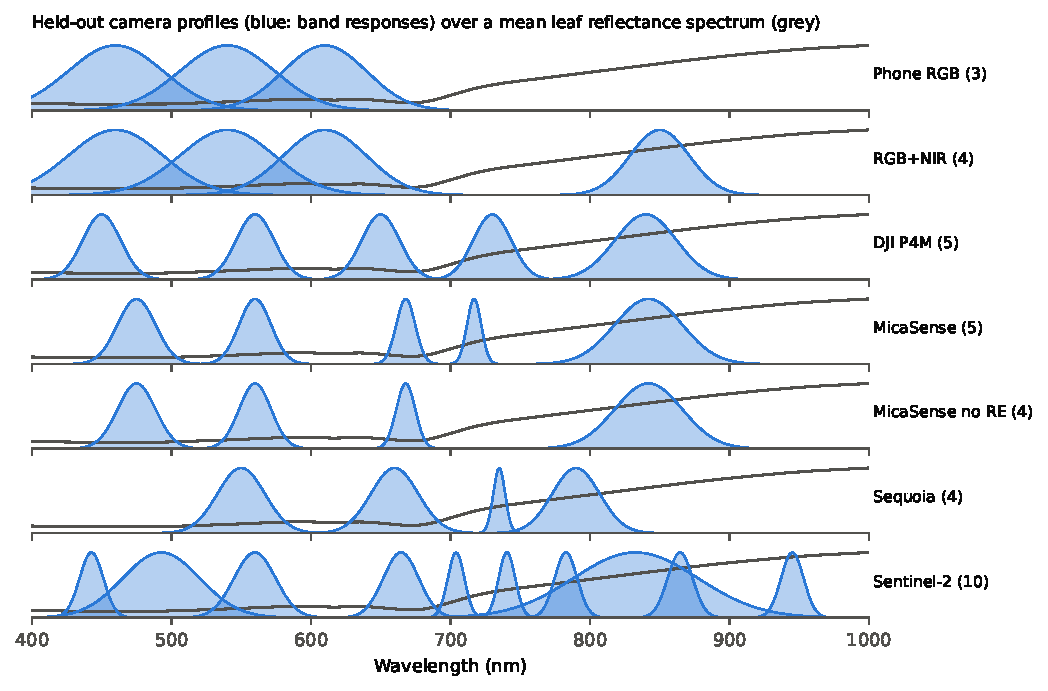
\includegraphics[width=\linewidth]{fig2_cameras.pdf}
\caption{Spectral responses of the seven held-out camera profiles over a mean leaf reflectance spectrum.}
\label{fig:cameras}
\end{figure}

\subsection{Stochastic Virtual Camera Training (SVCT)}
Fig.~\ref{fig:method} summarises the method. SVCT changes only the training data distribution and the first layer of
the network.

\textbf{Virtual camera sampler.} With probability $p_{full}=0.3$ a mini-batch uses all 204 bands. Otherwise a virtual
camera is drawn from a mixture of three families: \emph{RGB-like} (three wide visible bands with centres in
430--490, 510--570 and 580--650\,nm, FWHM 40--100\,nm, plus a NIR band with probability 0.3; weight 0.45),
\emph{multispectral} (4--5 bands drawn from blue, green, red, red-edge and NIR slots with jittered centres, FWHM
10--60\,nm; weight 0.35) and \emph{random} (3--12 bands anywhere in 400--1000\,nm, FWHM 10--100\,nm; weight 0.2). A
virtual camera whose band centres all lie within 15\,nm of a held-out profile with the same number of bands is rejected,
so the test cameras are never practised.

\textbf{Calibration errors.} With probability 0.5 per sample, the rendered bands receive a per-band gain
($0.8$--$1.25$), offset ($\pm0.02$) and Gaussian noise at a random signal-to-noise ratio of 20--50\,dB.

\textbf{Normalisation for any camera.} Each input band is standardised. For a camera with matrix $\mathbf{M}$, the band
means and variances follow directly from the training mean $\boldsymbol\mu$ and covariance $\boldsymbol\Sigma$ of the
204-band leaf pixels: $\boldsymbol\mu_{\mathbf M}=\mathbf M\boldsymbol\mu$ and
$\boldsymbol\sigma^2_{\mathbf M}=\mathrm{diag}(\mathbf M\boldsymbol\Sigma\mathbf M^\top)$, so no data from a new camera is
needed.

\textbf{Input variant (a): wavelength-conditioned stem.} The first convolution of an ImageNet-pretrained ResNet18
\citep{he2016resnet,deng2009imagenet} is replaced by filters generated per band. For a band with centre $\lambda$ and
width $w$, the pretrained RGB filters are linearly interpolated at $\lambda$ (blue, green and red anchored at 460, 540
and 610\,nm) and a small MLP on Fourier features \citep{tancik2020fourier} of $(\lambda,w)$ adds a correction, scaled by
the RMS of the pretrained filters, whose last layer is initialised to zero:
$\mathbf W_b=\tfrac{3}{B}\big(\mathbf W^{RGB}(\lambda_b)+\mathrm{rms}\cdot g_\theta(\lambda_b,w_b)\big)$. With an RGB
camera the stem therefore starts exactly as the pretrained network.

\textbf{Input variant (b): interpolation.} The $B$ bands are linearly interpolated (with edge hold) back to the 204
training wavelengths using the camera's \emph{nominal} band centres, and a plain 204-band ResNet18 is used. This keeps
the architecture unchanged; only the training distribution differs from the baseline.

\textbf{Training objective.} Cross-entropy for cultivar plus mean squared error on standardised regression targets.
Consistency losses between two camera views of the same leaf were tried and removed (Section~\ref{sec:ablation}).

\begin{figure}[t]
\centering
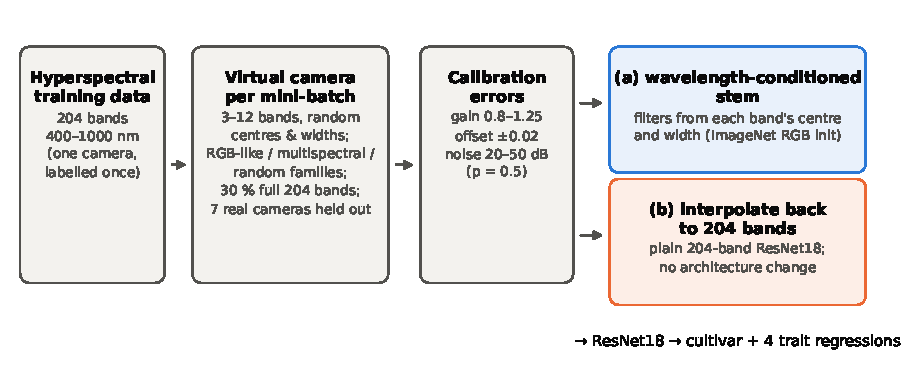
\includegraphics[width=\linewidth]{fig1_method.pdf}
\caption{Stochastic Virtual Camera Training. Each mini-batch is rendered through a random virtual camera with random
calibration errors; the bands enter the network either through a wavelength-conditioned stem (a) or after interpolation
to the 204 training wavelengths (b). At test time the real camera's bands and nominal band centres/widths are used.}
\label{fig:method}
\end{figure}

\subsection{Baselines and references}
\textbf{204-band model:} the same ResNet18 trained on all 204 bands (first convolution widened by spreading the averaged
RGB filters over the bands), applied to a new camera by interpolating its bands back to 204. This is what a user can do
today without retraining. \textbf{One model per camera:} a separate model trained on the simulated bands of each test
camera with the same labels; it needs labelled data for every camera and serves as an upper reference. We did not
include Hyve or CARL in this draft (Section~\ref{sec:limits}).

\subsection{Point-spectrum version for the real-camera tests}
DeepHS and Estrada provide one spectrum per sample, so we apply the same recipe to spectra: a two-layer MLP (256 units)
on interpolated bands (variant b), and a wavelength-aware set model that embeds every band as a token (value, Fourier
features of centre and width) with mean and max pooling (analogue of variant a). Models are trained only on the
training sensor (FX10, or the ASD spectrometer) with the same virtual camera sampler and calibration errors; the
held-out rule again excludes the seven camera profiles. For the Estrada MicaSense images, digital numbers are converted
to reflectance with a per-band linear empirical line fitted on the \emph{training} leaves only (similar to using a
reflectance panel; no trait labels are used). References are models trained on labelled data of the target camera
(Corning recordings; real MicaSense values) and, for Estrada, a model trained on \emph{simulated} MicaSense bands.

\subsection{Evaluation protocol}
Each HyperLeaf model is tested on the test plots under four conditions per held-out camera: \emph{ideal} (nominal
responses), \emph{drift} (band centres shifted up to $\pm$10\,nm and widths changed up to $\pm$25\%, averaged over three
draws, while the model is told the nominal values), \emph{calibration error} (gain, offset, noise as above) and both.
We also test on 20 random unseen virtual cameras and on the full 204 bands. Metrics are accuracy and macro-F1 for
classification and $R^2$ for regression. We summarise the gap to the camera-specific models as
\emph{gap closed} $=(\text{SVCT}-\text{baseline})/(\text{own-camera model}-\text{baseline})$. DeepHS and Estrada use
fruit- and leaf-grouped 5-fold cross-validation repeated with 3 seeds (15 folds; mean $\pm$ standard deviation).

\subsection{Implementation}
PyTorch with timm \citep{wightman2019timm}; AdamW \citep{loshchilov2019adamw} (learning rate $3\times10^{-4}$, weight
decay 0.05), cosine schedule, batch size 32, mixed precision, input upscaled $2\times$, flips, small shifts, per-band
gain and noise augmentation, single NVIDIA T4 GPU (Kaggle). The baseline trains for up to 50 epochs (early stopping
patience 12); SVCT for up to 150 epochs (patience 50), selecting the checkpoint by validation accuracy and MSE averaged
over the full camera and five fixed virtual validation cameras (never the held-out profiles). Point-spectrum models use
AdamW ($10^{-3}$), batch 64, 200 (DeepHS) or 150 (Estrada) epochs on CPU. Code, camera profiles, splits and all result
files are available at \url{https://github.com/ShahnawazQ007/one-model-many-camera}.

% =====================================================================
\section{Results}

\subsection{Reference model on the original camera}
Table~\ref{tab:baseline} shows the 204-band models on the official split. Upscaling the input and stronger augmentation
raised cultivar accuracy from 0.730 to 0.821; ConvNeXt-T \citep{liu2022convnext} was not better. We use the ResNet18
with $2\times$ input as the reference. Stomatal conductance is not predictable ($R^2\le0.11$) and is not discussed
further.

\begin{table}[t]
\centering\small
\caption{204-band models on HyperLeaf2024 (official split, test plots).}
\label{tab:baseline}
\begin{tabular}{@{}lcccccc@{}}
\toprule
 & \multicolumn{2}{c}{Cultivar} & \multicolumn{4}{c}{$R^2$} \\
\cmidrule(lr){2-3}\cmidrule(l){4-7}
Model & Acc. & F1 & Grain & $g_{sw}$ & $\Phi_{PSII}$ & Fert. \\
\midrule
ResNet18, 204 bands & 0.730 & 0.705 & 0.712 & 0.114 & 0.407 & 0.774 \\
ResNet18, $2\times$ input, strong aug.\ (reference) & 0.821 & 0.805 & 0.584 & 0.077 & 0.524 & 0.759 \\
ConvNeXt-T, $2\times$ input, strong aug. & 0.768 & 0.764 & 0.714 & 0.037 & 0.471 & 0.785 \\
\bottomrule
\end{tabular}

\end{table}

\subsection{The camera gap}
Applied to the seven simulated cameras, the 204-band model loses most of its value (Table~\ref{tab:main}, first row;
Fig.~\ref{fig:percamera}): mean cultivar accuracy falls from 0.821 to 0.522 (0.360 for the phone, close to the 0.25
chance level), and the mean $R^2$ becomes negative for fertilizer ($-0.364$), grain weight ($-0.685$) and $\Phi_{PSII}$
($-0.562$), i.e.\ worse than predicting the mean. Models trained on each camera's own bands, however, reach 0.757
cultivar accuracy and 0.765 fertilizer $R^2$ on average (0.795 and 0.720 for the phone). The information is therefore
present in a few bands; the failure is that of the model, not of the camera.

\subsection{One SVCT model on seven unseen cameras}
Table~\ref{tab:main} and Fig.~\ref{fig:percamera} show the final SVCT models. With interpolation, one model reaches
0.732 mean cultivar accuracy (90\% of the gap closed; phone RGB 0.768 vs.\ 0.795 for a phone-specific model). With the
wavelength-conditioned stem, regression is best: fertilizer $R^2$ 0.582 (84\% of the gap), grain weight 0.528 (88\%)
and $\Phi_{PSII}$ 0.254 (83\%), and every camera has a positive fertilizer $R^2$. Both variants are robust: with band
drift and calibration error together, cultivar accuracy drops by only 0.03 and fertilizer $R^2$ by 0.06--0.12. On 20
random unseen virtual cameras the stem variant gives 0.664 $\pm$ 0.075 cultivar accuracy and 0.513 $\pm$ 0.201
fertilizer $R^2$, and the interpolation variant 0.705 $\pm$ 0.099 and 0.417 $\pm$ 0.231.

The price is paid on the original camera: on the full 204 bands, SVCT reaches 0.660--0.689 cultivar accuracy and
0.589--0.629 fertilizer $R^2$, versus 0.821 and 0.759 for the specialised 204-band model. In practice the specialised
model should be kept for the hyperspectral camera and the SVCT model used for every other camera.

\begin{table}[t]
\centering\small
\setlength{\tabcolsep}{3.5pt}
\caption{Mean over the seven held-out camera profiles (HyperLeaf2024, official split). Bold: best single model without
camera-specific training. $^\ast$Needs labelled data from each camera (upper reference). Gap closed relative to the
own-camera models.}
\label{tab:main}
\resizebox{\linewidth}{!}{\begin{tabular}{@{}lcccccccc@{}}
\toprule
 & \multicolumn{4}{c}{Ideal cameras} & \multicolumn{2}{c}{Drift + calib.\ error} & \multicolumn{2}{c}{Full 204 bands} \\
\cmidrule(lr){2-5}\cmidrule(lr){6-7}\cmidrule(l){8-9}
Method & Cult.\ acc. & Fert.\ $R^2$ & Grain $R^2$ & $\Phi_{PSII}$ $R^2$ & Cult. & Fert. & Cult. & Fert. \\
\midrule
204-band model, bands interpolated & 0.522 & $-$0.364 & $-$0.685 & $-$0.562 & 0.505 & $-$0.488 & 0.821 & 0.759 \\
SVCT + wavelength stem (ours) & 0.670 & \textbf{0.582} & \textbf{0.528} & \textbf{0.254} & 0.640 & 0.462 & 0.660 & 0.589 \\
SVCT + interpolation (ours) & \textbf{0.732} & 0.468 & 0.429 & 0.227 & 0.703 & 0.409 & 0.689 & 0.629 \\
One model per camera$^\ast$ & 0.757 & 0.765 & 0.694 & 0.427 & -- & -- & -- & -- \\
\midrule
\quad gap closed, wavelength stem & 63\% & 84\% & 88\% & 83\% & & & & \\
\quad gap closed, interpolation & 90\% & 74\% & 81\% & 80\% & & & & \\
\bottomrule
\end{tabular}
}
\end{table}

\begin{figure}[t]
\centering
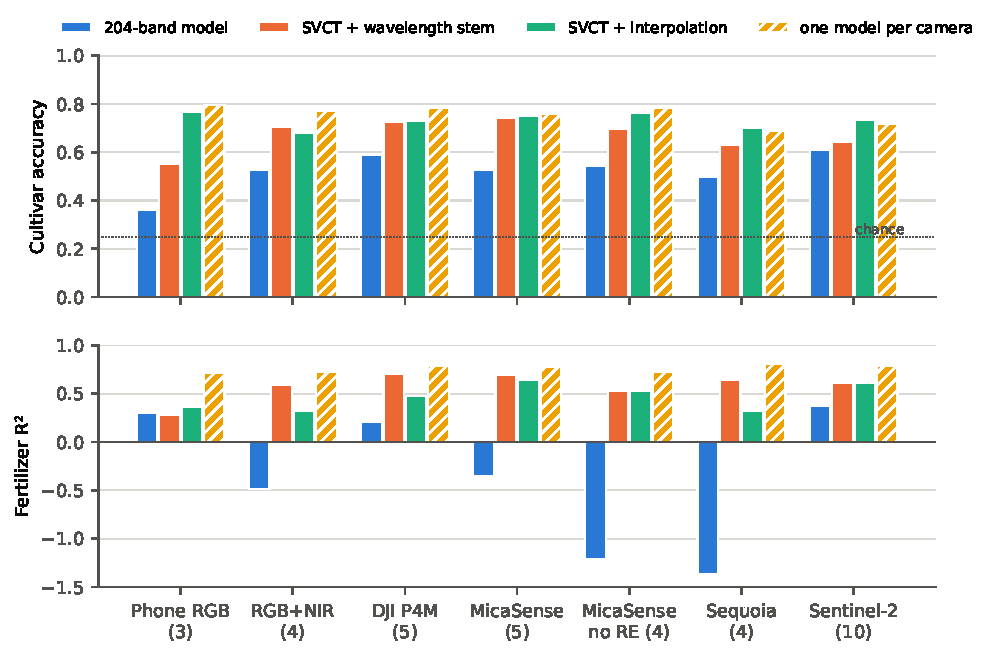
\includegraphics[width=\linewidth]{fig3_per_camera.pdf}
\caption{Per-camera results (ideal cameras). Hatched: one model trained per camera (needs labelled data from that camera).
Dotted line: chance level for cultivar (0.25).}
\label{fig:percamera}
\end{figure}

\subsection{What mattered during development}
\label{sec:ablation}
Table~\ref{tab:ablation} lists the three development rounds, all evaluated on the same held-out cameras. Two
observations shaped the final method. First, consistency losses between two camera views of the same leaf, either
symmetric or as distillation from the full-band view, consistently \emph{hurt} cultivar accuracy (0.502 vs.\ 0.639 in
round~1; 0.551 vs.\ 0.664 in round~2) while helping regression only slightly, so they were removed. Second, a structured
sampler that practises the \emph{types} of real cameras (RGB-like and multispectral layouts) without copying them, a
higher share of full-band batches and longer training (150 epochs) raised the stem variant from 0.639 to 0.670 cultivar
accuracy and from 0.456 to 0.582 fertilizer $R^2$. The method was frozen after round~3; these settings are used for all
other experiments.

\begin{table}[t]
\centering\scriptsize
\setlength{\tabcolsep}{3pt}
\caption{Development rounds (official split; mean over the seven held-out cameras, ideal conditions).}
\label{tab:ablation}
\begin{tabular}{@{}clcccccc@{}}
\toprule
 & & \multicolumn{4}{c}{7 held-out cameras (ideal)} & \multicolumn{2}{c}{204 bands} \\
\cmidrule(lr){3-6}\cmidrule(l){7-8}
Round & Variant & Cult. & Fert. & Grain & $\Phi_{PSII}$ & Cult. & Fert. \\
\midrule
1 & two views + symmetric consistency (w=1), uniform sampler & 0.502 & 0.480 & 0.464 & 0.203 & 0.562 & 0.543 \\
1 & same, without consistency & 0.639 & 0.456 & 0.356 & 0.285 & 0.707 & 0.609 \\
1 & same as first, interpolation instead of stem & 0.556 & 0.377 & 0.366 & 0.238 & 0.572 & 0.594 \\
2 & teacher distillation (w=0.5), structured sampler & 0.551 & 0.526 & 0.508 & 0.226 & 0.709 & 0.392 \\
2 & structured sampler, no consistency & 0.664 & 0.527 & 0.455 & 0.322 & 0.701 & 0.608 \\
2 & teacher distillation, interpolation & 0.647 & 0.418 & 0.387 & 0.234 & 0.645 & 0.681 \\
3 & final: no consistency, $p_{full}$=0.3, phone-weighted sampler, 150 ep. & 0.670 & 0.582 & 0.528 & 0.254 & 0.660 & 0.589 \\
3 & final, interpolation instead of stem & 0.732 & 0.468 & 0.429 & 0.227 & 0.689 & 0.629 \\
\bottomrule
\end{tabular}

\end{table}

\subsection{Cross-validation on HyperLeaf2024}
\label{sec:cv}
The official test set contains only a few plots, so the frozen settings are repeated with plot-grouped 5-fold
cross-validation (Table~\ref{tab:cv}). \todo{Step 9 is running at the time of writing; this table and the paragraph will
be updated with mean $\pm$ s.d.\ over the folds and the number of folds in which each SVCT variant beats the baseline.}

\begin{table}[t]
\centering\small
\setlength{\tabcolsep}{4pt}
\caption{Plot-grouped cross-validation on HyperLeaf2024 (mean $\pm$ s.d.\ over folds of the mean over the seven held-out
cameras).}
\label{tab:cv}
% Step 9 still running: placeholders
\begin{tabular}{@{}lccccc@{}}
\toprule
 & \multicolumn{3}{c}{Ideal cameras} & \multicolumn{2}{c}{Drift + calib.\ error} \\
\cmidrule(lr){2-4}\cmidrule(l){5-6}
Method & Cult.\ acc. & Fert.\ $R^2$ & Grain $R^2$ & Cult. & Fert. \\
\midrule
204-band model, bands interpolated & \pending & \pending & \pending & \pending & \pending \\
SVCT + wavelength stem (ours) & \pending & \pending & \pending & \pending & \pending \\
SVCT + interpolation (ours) & \pending & \pending & \pending & \pending & \pending \\
\bottomrule
\end{tabular}

\end{table}

\subsection{A real second camera: fruit (FX10 $\rightarrow$ Corning)}
Table~\ref{tab:deephs} and Fig.~\ref{fig:real}a show the DeepHS results. Trained only on FX10 spectra, the plain model
loses much on the real Corning camera: fruit-type accuracy 0.838 and sugar $R^2$ 0.547, while its firmness $R^2$ becomes
negative ($-0.364$). SVCT trained on the same FX10 data reaches 0.971 fruit accuracy and a sugar $R^2$ of 0.794, the same
as a model trained on labelled Corning data (0.793), and recovers most of the firmness skill (0.463 vs.\ 0.566). When the
Corning recordings are further reduced to the seven camera profiles, the plain model collapses (sugar $R^2$ 0.01) while
SVCT keeps 0.65. On the training camera SVCT loses nothing (sugar 0.799 vs.\ 0.773). Ripeness is difficult for every
model, including the one trained on Corning (about 0.58), which points to a limit of the labels rather than of the
camera.

\begin{table}[t]
\centering\scriptsize
\setlength{\tabcolsep}{4pt}
\caption{DeepHS fruit: models trained on Specim FX10 spectra, tested on unseen fruits (fruit-grouped 5-fold CV
$\times$ 3 seeds, mean $\pm$ s.d.). $^\ast$Trained on labelled Corning recordings.}
\label{tab:deephs}
\begin{tabular}{@{}lcccc@{}}
\toprule
Model & Fruit acc. & Ripeness acc. & Sugar $R^2$ & log-firmness $R^2$ \\
\midrule
\multicolumn{5}{@{}l}{\textit{Same camera (FX10)}} \\
\quad Plain MLP (FX10 only) & 0.982 $\pm$ 0.021 & 0.630 $\pm$ 0.103 & 0.773 $\pm$ 0.115 & 0.584 $\pm$ 0.230 \\
\quad SVCT, interpolation (FX10 only) & 0.979 $\pm$ 0.018 & 0.583 $\pm$ 0.048 & 0.799 $\pm$ 0.074 & 0.552 $\pm$ 0.186 \\
\quad SVCT, wavelength tokens (FX10 only) & 0.983 $\pm$ 0.025 & 0.589 $\pm$ 0.057 & 0.766 $\pm$ 0.081 & 0.568 $\pm$ 0.218 \\
\multicolumn{5}{@{}l}{\textit{Real Corning camera}} \\
\quad Plain MLP (FX10 only) & 0.838 $\pm$ 0.110 & 0.558 $\pm$ 0.051 & 0.547 $\pm$ 0.293 & $-$0.364 $\pm$ 0.623 \\
\quad SVCT, interpolation (FX10 only) & 0.971 $\pm$ 0.034 & 0.576 $\pm$ 0.036 & 0.794 $\pm$ 0.065 & 0.463 $\pm$ 0.244 \\
\quad SVCT, wavelength tokens (FX10 only) & 0.961 $\pm$ 0.051 & 0.589 $\pm$ 0.068 & 0.731 $\pm$ 0.123 & 0.455 $\pm$ 0.341 \\
\quad Trained on Corning labels$^\ast$ & 0.995 $\pm$ 0.009 & 0.580 $\pm$ 0.095 & 0.793 $\pm$ 0.092 & 0.566 $\pm$ 0.251 \\
\multicolumn{5}{@{}l}{\textit{Real Corning, reduced to the 7 camera profiles (mean)}} \\
\quad Plain MLP (FX10 only) & 0.531 $\pm$ 0.117 & 0.444 $\pm$ 0.080 & 0.014 $\pm$ 0.459 & $-$3.858 $\pm$ 2.847 \\
\quad SVCT, interpolation (FX10 only) & 0.934 $\pm$ 0.033 & 0.543 $\pm$ 0.041 & 0.651 $\pm$ 0.078 & 0.403 $\pm$ 0.155 \\
\quad SVCT, wavelength tokens (FX10 only) & 0.945 $\pm$ 0.023 & 0.574 $\pm$ 0.052 & 0.648 $\pm$ 0.120 & 0.376 $\pm$ 0.320 \\
\multicolumn{5}{@{}l}{\textit{FX10, reduced to the 7 camera profiles (mean)}} \\
\quad Plain MLP (FX10 only) & 0.716 $\pm$ 0.095 & 0.412 $\pm$ 0.082 & 0.098 $\pm$ 0.327 & $-$2.742 $\pm$ 2.134 \\
\quad SVCT, interpolation (FX10 only) & 0.947 $\pm$ 0.024 & 0.550 $\pm$ 0.036 & 0.697 $\pm$ 0.087 & 0.459 $\pm$ 0.152 \\
\quad SVCT, wavelength tokens (FX10 only) & 0.960 $\pm$ 0.028 & 0.573 $\pm$ 0.045 & 0.705 $\pm$ 0.096 & 0.469 $\pm$ 0.239 \\
\bottomrule
\end{tabular}

\end{table}

\subsection{A real drone camera: leaves (spectrometer $\rightarrow$ MicaSense)}
On simulated cameras the Estrada results repeat the HyperLeaf picture (Table~\ref{tab:estrada}): the plain model gives
negative $R^2$ for chlorophyll and water content, while SVCT with wavelength tokens reaches 0.733 and 0.564 and 0.843
crop accuracy. On the real MicaSense images (Fig.~\ref{fig:real}b) both SVCT variants improve every task over the plain model
(best variant: chlorophyll $R^2$ $-0.002\rightarrow0.465$, crop accuracy $0.457\rightarrow0.543$), but stays far below a model trained
on labelled MicaSense data (crop 0.927, chlorophyll 0.800). This gap is not specific to SVCT: even a model trained on
\emph{simulated} MicaSense bands of the same leaves reaches only 0.593 crop accuracy on the real images. The reason is
radiometric: after the empirical-line conversion, the agreement between real and simulated band values is low
($R^2$ 0.04 blue, 0.34 green, 0.08 red, 0.61 red edge, 0.01 NIR), because the released images are uncalibrated digital
numbers without panel or exposure information. Unlike on fruit, SVCT also costs accuracy on the original spectrometer
data here (interpolation variant: drying stage 0.899 $\rightarrow$ 0.681; water $R^2$ 0.934 $\rightarrow$ 0.750).

\begin{table}[t]
\centering\scriptsize
\setlength{\tabcolsep}{4pt}
\caption{Estrada leaves: models trained on ASD spectrometer spectra (400--1000\,nm), tested on unseen leaves
(leaf-grouped 5-fold CV $\times$ 3 seeds, mean $\pm$ s.d.). $^\S$Simulated from the spectrometer (one model per camera,
simulated). $^\ast$Trained on labelled real MicaSense values.}
\label{tab:estrada}
\begin{tabular}{@{}lcccc@{}}
\toprule
Model & Crop acc. & Stage acc. & Chlorophyll $R^2$ & Water (FMC) $R^2$ \\
\midrule
\multicolumn{5}{@{}l}{\textit{Same sensor (spectrometer, 400--1000 nm)}} \\
\quad Plain MLP (spectrometer only) & 0.980 $\pm$ 0.007 & 0.899 $\pm$ 0.017 & 0.860 $\pm$ 0.023 & 0.934 $\pm$ 0.009 \\
\quad SVCT, interpolation & 0.924 $\pm$ 0.013 & 0.681 $\pm$ 0.020 & 0.812 $\pm$ 0.024 & 0.750 $\pm$ 0.020 \\
\quad SVCT, wavelength tokens & 0.912 $\pm$ 0.016 & 0.647 $\pm$ 0.022 & 0.798 $\pm$ 0.029 & 0.708 $\pm$ 0.019 \\
\multicolumn{5}{@{}l}{\textit{Real MicaSense camera}} \\
\quad Plain MLP (spectrometer only) & 0.457 $\pm$ 0.044 & 0.198 $\pm$ 0.028 & $-$0.002 $\pm$ 0.243 & $-$0.154 $\pm$ 0.114 \\
\quad SVCT, interpolation & 0.524 $\pm$ 0.031 & 0.275 $\pm$ 0.016 & 0.465 $\pm$ 0.056 & 0.149 $\pm$ 0.086 \\
\quad SVCT, wavelength tokens & 0.543 $\pm$ 0.035 & 0.271 $\pm$ 0.017 & 0.425 $\pm$ 0.041 & 0.192 $\pm$ 0.046 \\
\quad Trained on simulated MicaSense$^\S$ & 0.593 $\pm$ 0.051 & 0.270 $\pm$ 0.018 & 0.356 $\pm$ 0.076 & $-$0.115 $\pm$ 0.110 \\
\quad Trained on real MicaSense labels$^\ast$ & 0.927 $\pm$ 0.009 & 0.525 $\pm$ 0.028 & 0.800 $\pm$ 0.017 & 0.514 $\pm$ 0.033 \\
\multicolumn{5}{@{}l}{\textit{Simulated, 7 camera profiles (mean)}} \\
\quad Plain MLP (spectrometer only) & 0.522 $\pm$ 0.026 & 0.176 $\pm$ 0.014 & $-$0.366 $\pm$ 0.371 & $-$0.633 $\pm$ 0.141 \\
\quad SVCT, interpolation & 0.810 $\pm$ 0.017 & 0.515 $\pm$ 0.016 & 0.721 $\pm$ 0.027 & 0.539 $\pm$ 0.026 \\
\quad SVCT, wavelength tokens & 0.843 $\pm$ 0.017 & 0.539 $\pm$ 0.020 & 0.733 $\pm$ 0.027 & 0.564 $\pm$ 0.026 \\
\bottomrule
\end{tabular}

\end{table}

\begin{figure}[t]
\centering
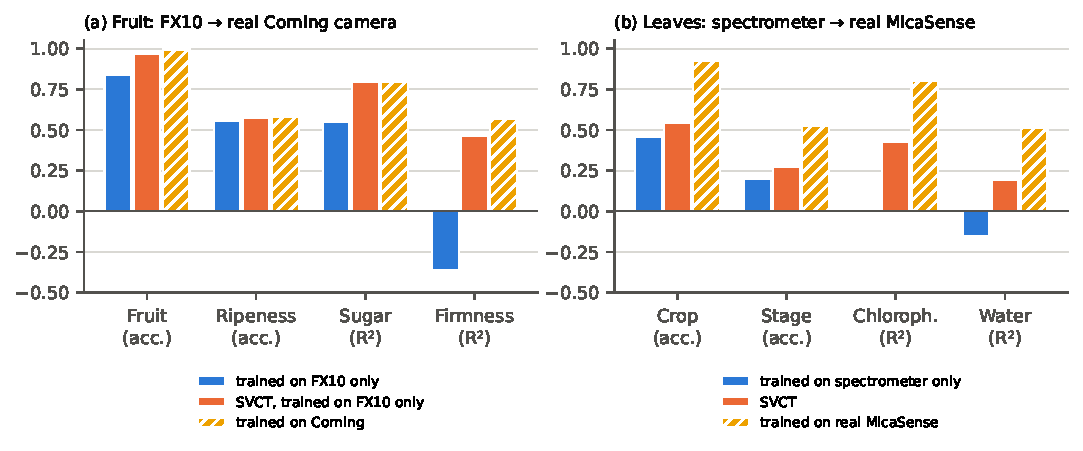
\includegraphics[width=\linewidth]{fig4_real_cameras.pdf}
\caption{Tests on real second cameras. (a) DeepHS: trained on Specim FX10, tested on the real Corning microHSI 410.
(b) Estrada: trained on an ASD spectrometer, tested on real (uncalibrated) MicaSense images. Hatched: trained on
labelled data of the target camera.}
\label{fig:real}
\end{figure}

% =====================================================================
\section{Discussion}
\textbf{A training distribution, not an architecture.} The largest gain came from what the network sees during
training. The interpolation variant uses an unchanged 204-band ResNet18 and is the best classifier on unseen cameras;
it can be applied to any existing model with a re-training run and no new data. The wavelength-conditioned stem is better
for the physiological regressions (fertilizer, grain weight, $\Phi_{PSII}$), consistent with the observation that these
traits depend more on spectral detail \citep{laprade2024hyperleaf}. Whether this ordering holds beyond one split is the
purpose of the cross-validation in Section~\ref{sec:cv}.

\textbf{Consistency is not free.} Forcing two camera views of a leaf to agree is an intuitive regulariser, but it
consistently lowered cultivar accuracy. A plausible reason is that a phone view and a full-band view legitimately carry
different information; requiring identical outputs pulls the full-band representation towards the weakest camera.

\textbf{Simulation versus reality.} The simulator reproduces a second real hyperspectral camera well (band correlations
0.94--0.998), and on that camera SVCT matches a camera-specific model for sugar. The real drone test shows the other
side: when the target camera's radiometry is unknown, both SVCT and a model trained on simulated drone bands fall far
short of a model trained on the real images. Radiometric calibration (a reflectance panel) is therefore a precondition
for any simulation-trained model, not a detail.

\textbf{Practical use.} A user needs only the band centres and widths of their camera, which are published by
manufacturers. The camera-specific models remain better and should be used when labelled data from the target camera
exist; SVCT is aimed at the much more common case where they do not.

\subsection{Limitations}
\label{sec:limits}
(i) The main HyperLeaf results come from the official split with one seed; cross-validation is in progress
(Section~\ref{sec:cv}) and statistical tests are still to be added. (ii) The seven HyperLeaf test cameras are simulated
with Gaussian responses; the phone and RGB+NIR profiles are approximate. (iii) HyperLeaf comes from one field and season,
so we claim robustness to sensor shift only. (iv) SVCT lowers accuracy on the original hyperspectral camera
(Table~\ref{tab:main}); a two-model deployment avoids this. (v) Hyve, CARL and adaptation baselines were not run for
this draft. (vi) The real-camera tests use one spectrum per sample (point spectra), not full images.

% =====================================================================
\section{Conclusion}
Training with random virtual cameras turns a hyperspectral plant model that fails on cheaper cameras into one model
that works reasonably on seven unseen camera profiles, closing most of the gap to models trained separately for each
camera without any data from those cameras. On a real second hyperspectral camera, it matches a camera-specific model
for fruit sugar content. Remaining gaps are on the original camera and on uncalibrated real drone images, where
radiometric calibration is the bottleneck. Next steps are the cross-validated comparison with Hyve and CARL, measured
camera responses, and field drone data with reflectance panels.

\section*{Data and code availability}
HyperLeaf2024, DeepHS Fruit and the Estrada leaf dataset are public. Code, camera profiles, data splits and all result
files: \url{https://github.com/ShahnawazQ007/one-model-many-camera}.

\section*{Declaration of competing interest}
The author declares no competing interests.

\bibliographystyle{\bibsty}
\bibliography{refs}

\end{document}
